\centering
\subsection*{Einführung}
Der Zähler besteht aus einem Geiger-Müller-Rohr, das in einem Metallgehäuse untergebracht ist. 
Das Rohr ist mit einem Gasgemisch aus Argon und Ethanol gefüllt und mit einem Hochspannungsgenerator verbunden. 
Wenn ionisierende Strahlung auf das Rohr trifft, wird das Gas ionisiert und es kommt zu einer Entladung, die als Stromimpuls gemessen wird. 
Der Stromimpuls wird verstärkt und anschließend von einem Mikrocontroller wie dem Arduino ausgewertet.
\subsection*{Projektaufbau}
Die elektronischen Komponenten, die für den Bau des Geiger-Müller-Zählers benötigt werden, sind ein Arduino, ein Geiger-Müller-Rohr, ein Hochspannungsgenerator, ein Verstärker und ein Display.

Das Geiger-Müller-Rohr wandelt die ionisierende Strahlung in einen elektrischen Impuls um, der vom Verstärker verstärkt wird. 
Der Hochspannungsgenerator erzeugt eine Hochspannung, die das Geiger-Müller-Rohr ionisiert. 
Das Display zeigt die Anzahl der gemessenen Impulse pro Sekunde an.
Zusätzlich wird für die Energieauflösung entweder ein Filterradsystem konstruiert oder mit einem Multichannel-Analysator von der Stärke der Pulse auf die Energie der Strahlung zurückgeschlossen.
Dies ist jedoch nicht in der Aufbauskizze eingzeichnet, da diese nur schematisch ist und während der Projektdurchführung angepasst wird. 

\begin{figure}[H]
    \centering
    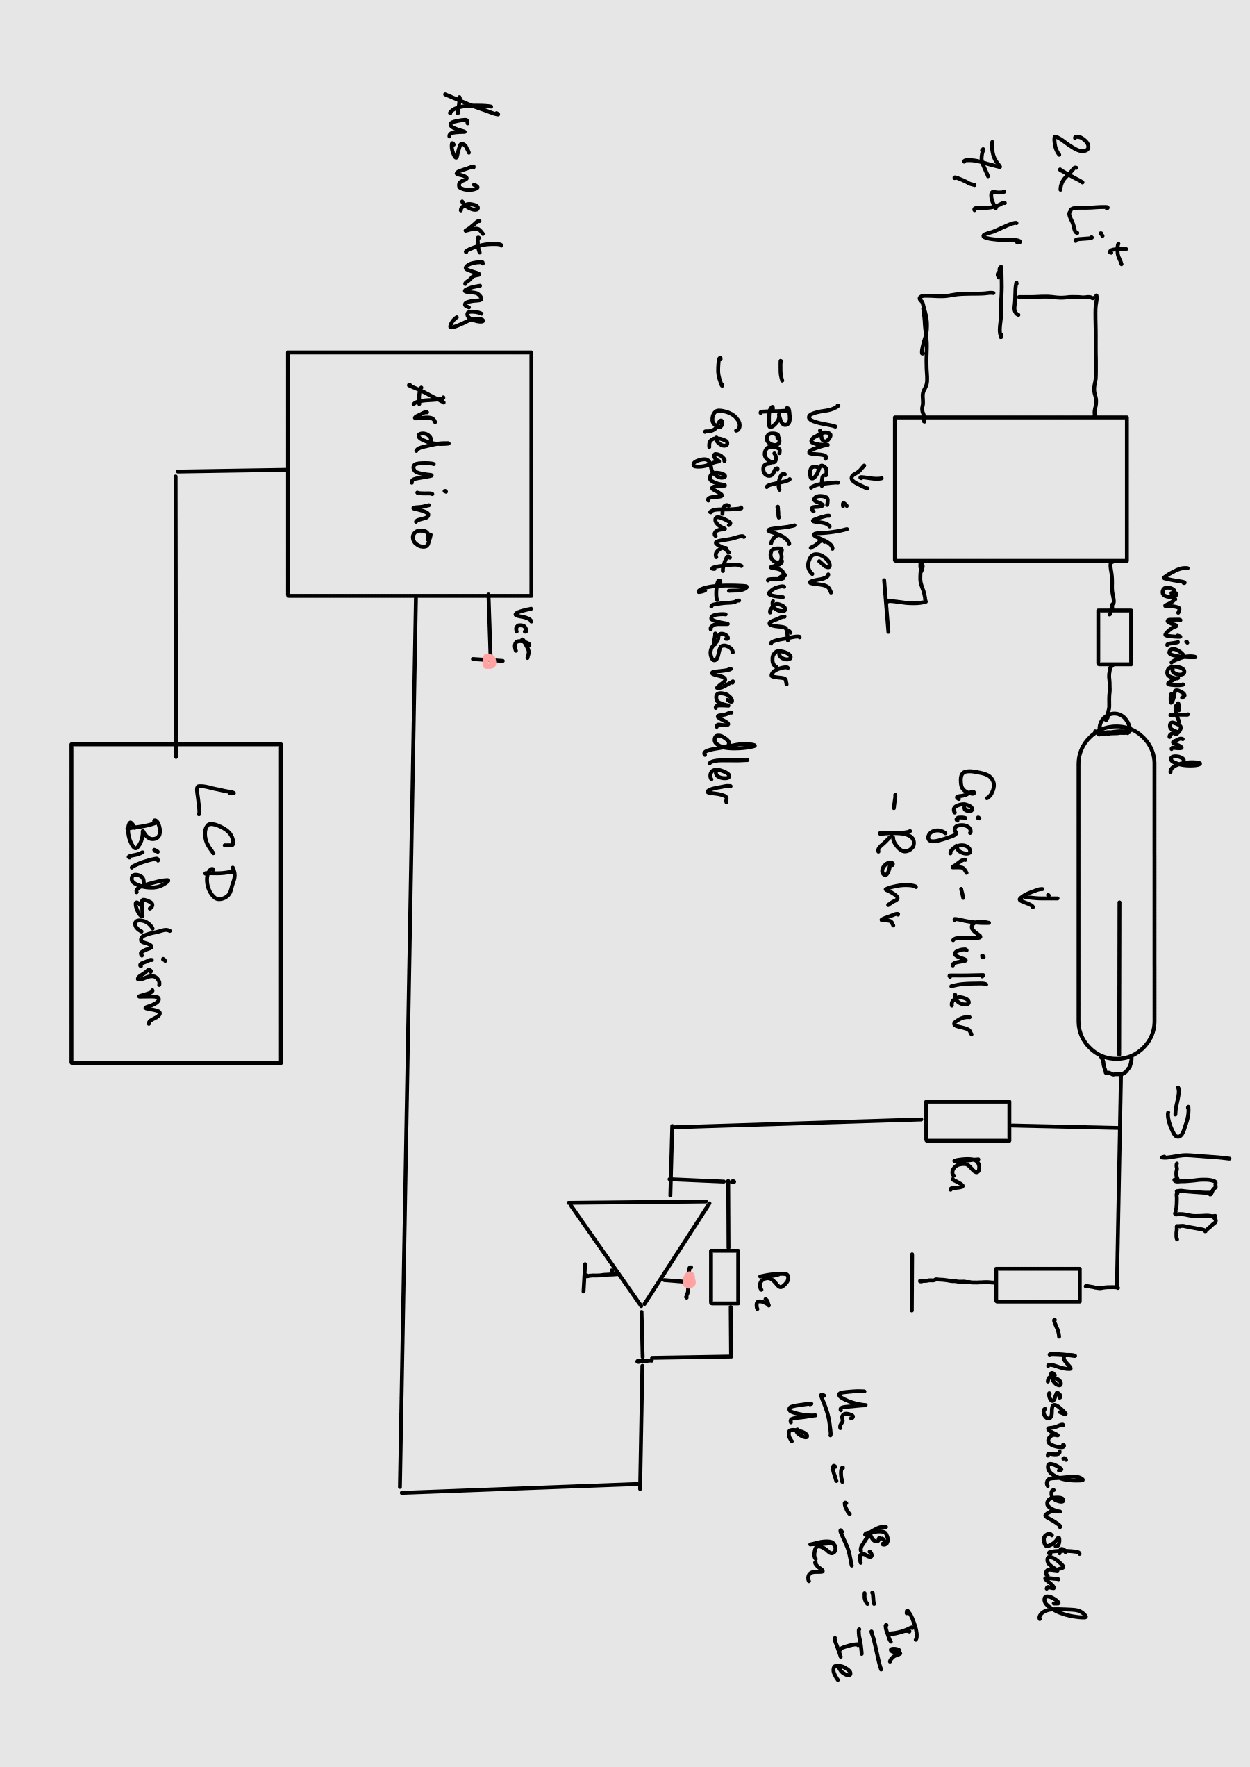
\includegraphics[angle=90, width=0.5\textwidth]{Geiger.pdf}
    \caption{Schematischer Aufbau, vermutlich mehrere Operationsverstärker zusammengeschalten, Der gesammte Aufbau würde sich in einem Plastikgehäuse befinden und mittels Tasten oder Touchbildschirm bedienen lassen.}
\end{figure}
\subsection*{Physikalische Anforderungen}
\begin{itemize}
    \item Empfindlichkeit: Der Geigerzähler sollte in der Lage sein, selbst sehr geringe Mengen von ionisierender Strahlung zu erkennen und zu messen. ( Wahl des Füllgases entscheidend)

    \item Stabilität: Der Zähler sollte bei wiederholten Messungen konsistente Ergebnisse liefern.(Auswertungselektronik soll Taktraten des Arduinos berücksichtigen )
    
    \item Linearität: Die Zählrate sollte proportional zur Intensität der Strahlung sein, um genaue Messungen zu ermöglichen.(Stabile Versorgungspannung)
    \item Energieauflösung: Der Zähler sollte in der Lage sein, Strahlung in verschiedene Energiebereiche aufzulösen, um verschiedene Arten von Strahlung zu identifizieren. (Die Schwellenergie wird durch die Art des Füllgases beinflusst.)
\end{itemize}

\subsection*{Komponenten und Kosten}
\begin{table}[H]
    \label{tab:eins}
    \centering
    \caption{Komponenten und Kosten}
    \begin{tabular}{cc} \hline
     Komponente& Kosten / Euro\\ \hline
     Arduino& vorhanden\\ \hline
     GM-Zählrohr& $\approx$ 60  \\ \hline
     OPV's& $\approx$ 1 - 10 \\ \hline
     DC-DC Boost Wandler& $\approx$ 20  \\ \hline
     Widerstände-Kit&$\approx$ 10 \\ \hline
     Lithium-Ionen Akkus & $\approx$ 10 - 20 \\ \hline
     Display & $\approx$ 10 - 20 \\ \hline \hline
     Summe & 110 - 140 \\ \hline
    \end{tabular}
    \end{table}
\subsection*{Software}
Arduino IDE, Python vielleicht

\subsection*{Aufwandsabschätzung}
\begin{table}[H]
    \label{tab:zwei}
    \centering
    \caption{Aufandsabschätzung}
    \begin{tabular}{cc} \hline
    Arbeitspaket & Aufwand / h \\ \hline
    Konzipierung der Schaltung &  20 - 30 \\ \hline
    Aufbau/Test & 20 - 30\\ \hline
    Messoptimierung & 20 - 30  \\ \hline
    Auswertungssoftware & 10 -20 \\ \hline
    Gehäuse Design & 5  \\ \hline
    Debugging & 50 - 100 \\ \hline
    UI/Ansteuerung  & 10 - 20  \\ \hline \hline
    Summe & 135 - 235  \\ \hline
    \end{tabular}
    \end{table}